\documentclass{sigchi-ext}
% Please be sure that you have the dependencies (i.e., additional
% LaTeX packages) to compile this example.
\usepackage[T1]{fontenc}
\usepackage{textcomp}
\usepackage[scaled=.92]{helvet} % for proper fonts
\usepackage{graphicx} % for EPS use the graphics package instead
\usepackage{balance}  % for useful for balancing the last columns
\usepackage{booktabs} % for pretty table rules
\usepackage{ccicons}  % for Creative Commons citation icons
\usepackage{ragged2e} % for tighter hyphenation
\usepackage{todonotes}
\usepackage{subfig}

% \usepackage{marginnote} \usepackage[shortlabels]{enumitem}
% \usepackage{paralist}

%% EXAMPLE BEGIN -- HOW TO OVERRIDE THE DEFAULT COPYRIGHT STRIP --
% \copyrightinfo{Permission to make digital or hard copies of all or
% part of this work for personal or classroom use is granted without
% fee provided that copies are not made or distributed for profit or
% commercial advantage and that copies bear this notice and the full
% citation on the first page. Copyrights for components of this work
% owned by others than ACM must be honored. Abstracting with credit is
% permitted. To copy otherwise, or republish, to post on servers or to
% redistribute to lists, requires prior specific permission and/or a
% fee. Request permissions from permissions@acm.org.\\
% {\emph{CHI'14}}, April 26--May 1, 2014, Toronto, Canada. \\
% Copyright \copyright~2014 ACM ISBN/14/04...\$15.00. \\
% DOI string from ACM form confirmation}
%% EXAMPLE END

\title{StoAR: Blending Physical and Virtual Shopping Experiences through Augmented Reality}
\numberofauthors{5}
% Notice how author names are alternately typesetted to appear ordered
% in 2-column format; i.e., the first 4 autors on the first column and
% the other 4 auhors on the second column. Actually, it's up to you to
% strictly adhere to this author notation.

\author{%
	\alignauthor{%
		\textbf{Matt Whitlock}\\
		\affaddr{University of Colorado} \\
		\affaddr{Boulder, CO 80309, USA} \\
		\affaddr{matthew.whitlock@colorado.edu} }\alignauthor{%
		\textbf{Jed Brubaker}\\
		\affaddr{University of Colorado} \\
		\affaddr{Boulder, CO 80309, USA} \\
		\affaddr{jed.brubaker@colorado.edu} }\vfil \alignauthor{%
		\textbf{Ethan Hanner}\\
		\affaddr{University of Colorado} \\
		\affaddr{Boulder, CO 80309, USA} \\
		\affaddr{ethan.hanner@colorado.edu} }\alignauthor{%
		\textbf{Danielle Szafir}\\    
		\affaddr{University of Colorado} \\
		\affaddr{Boulder, CO 80309, USA} \\
		\affaddr{danielle.szafir@colorado.edu} }\vfil \alignauthor{%
		\textbf{Shaun Kane}\\
		\affaddr{University of Colorado} \\
		\affaddr{Boulder, CO 80309, USA} \\
		\affaddr{shaun.kane@colorado.edu} } }

% Paper metadata (use plain text, for PDF inclusion and later
% re-using, if desired)
\def\plaintitle{StoAR: Blending Physical and Virtual Shopping Experiences through Augmented Reality}
 \def\plainauthor{Matt Whitlock, Ethan Hanner, Shaun Kane,
  Jed Brubaker, Danielle Szafir}
\def\plainkeywords{Augmented Reality; Mixed Reality; Shopping.}
\def\plaingeneralterms{Documentation, Standardization}

%% Set up our PDF with metadata
\hypersetup{%
  pdftitle={\plaintitle}, pdfauthor={\plainauthor},
  pdfkeywords={\plainkeywords}, }

% \reversemarginpar%

\begin{document}

\maketitle

% Uncomment to disable hyphenation (not recommended)
% https://twitter.com/anjirokhan/status/546046683331973120
\RaggedRight{} 

% Do not change the page size or page settings.
\begin{abstract}
	Augmented reality systems allow designers to blend aspects of physical and virtual experiences; however, existing work provides little guidance for effectively merging parallel experiences. In this work, we use retail shopping as a case study to understand how user-centered design practices might enable designers to craft novel AR applications from existing parallel in-store and online experiences. Through a series of surveys, prototypes, and design evaluations, we work directly with target users to identify trade-offs of in-store and online shopping and derive a set of design considerations for how augmented reality might support consumer decision making in traditional retail environments. Our findings suggest that users perceive AR as an effective means for contextualized, at-a-glance access to critical information available in online shopping, such as price comparisons and review information, while retaining the convenience and immediacy of physical interactions with products from in-store experiences.  We also found preliminary evidence of how blending existing parallel experiences might inspire novel immersive interactions that transcend traditional retail experiences. \todo{this is too long}
%As much of store commerce has migrated online, consumers are growing to appreciate aspects of online shopping--in several ways more than the in-store experience.  Using the appropriate technology, one could effectively merge aspects of the in-store and online shopping experiences.  
%We present StoAR, a system that employs augmented reality to deliver an important subset of the online shopping experience without sacrificing aspects of the in-store experience which customers appreciate.  We have provided users with  
% We administered surveys and user tests throughout the design process.  We conclude that augmented reality is an effective vehicle to merge online and in-store shopping experiences, providing a novel means of customer engagement.

  %Abstracts should be about 150 words. Required.
\end{abstract}

\keywords{\plainkeywords}

\category{H.5.1}{Information interfaces and presentation}{Multimedia Information Systems: \textit{Artificial, augmented, and virtual realities}}
\section{Introduction}

The retail industry has shifted more of its commerce to the online realm.  Shoppers have the options do their shopping at in the store or to engage with that same store's online presence.  Retailers have adapted the online and in-store shopping experiences in ways that suit the needs of online and in-store shoppers respectively.  (TODO:  I THINK SOME OF THIS NEEDS LITERATURE BACKING; THIS IS BASED ON HUNCHES)  This leaves customers with a new dilemma--one which forces them to choose between the benefits of one shopping experience over the other, while accepting that experience's limitations.

We discuss the benefits and drawbacks of the online and in-store shopping experiences later in this paper, and find that the benefits of one experience tend to line up with the drawbacks of the other.  So with this work, we aim to merge previously parallel norms into a hybrid virtual and physical one which empowers users with important aspects of both.  Through StoAR, we propose that augmented reality via a head-mounted display is an appropriate medium in delivering this hybrid experience.

A good deal of research has been devoted to defining characteristics of an application for which augmented reality is applicable.  A hybrid retail experience matches many of the theoretical grounds laid out by previous work.  StoAR applies augmented reality head-mounted displays in the widely relatable retail domain, allowing for more widespread use of novel head-mounted display technology.


\section{Related Work}

Previous work applying augmented reality to retail shopping has focused on how designers and system architects properly utilize this novel technology. Ahn et al. employed augmented reality to promote health-oriented shopping\cite{ahn2015supporting}, and similarly, Cenieros et al. focused on environmentally-conscious shopping \cite{ceniceros2014augmented}. These and other works \cite{esser2016head,stoyanova2015comparison} discuss the influence augmented reality can have in a store environment. Context-awareness is a useful affordance provided by augmented reality.  Designers find that this ability to visually associate digital content with products increases customer empowerment, user efficiency in gathering information, and system influence \cite{kourouthanassis2007enhancing,olsson2013expected,zhu2004personalized}. Augmented reality application work has additionally focused on collaborative experiences and visualizations \cite{esser2016head,santos2016augmented,stoyanova2015comparison,truong2013today}. These efforts highlight the importance of context-awareness and visualization provided by augmented reality in providing new functionality. However, we engage in a user-centered design process to identify aspects of existing parallel experiences in order to merge those experiences to one that is useful and familiar.

\begin{marginfigure}
	\begin{minipage}{\marginparwidth}
		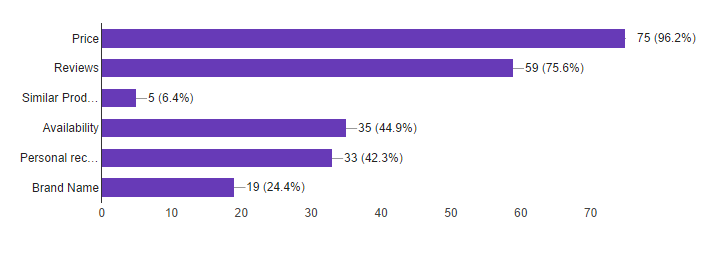
\includegraphics[width=0.9\columnwidth]{figures/ShoppingFactors}
		\caption{Phase One respondants identified price and reviews as the most critical factors in making their shopping decisions, while product comparisons---identified in later phases as ``highly useful''---were initially rated as least important. \textbf{DNS: Axis labels please!!! Turn into vertical chart s.t. it's legible as a margin fig. Also use full labels rather than ellipses. May have to reconstruct in powerpoint or inkscape}}
		\label{figures:ShoppingFactors}
	\end{minipage}
\end{marginfigure}

\todo[inline]{DNS: Do we have any insight into how current systems are designed? That may be a nice transition from conventional systems and this approach. MW: Not really. I can go through the work some more but most of the focus is on how the systems affect users.}

Much of this previous work has focused on mobile augmented reality (MAR). However, MAR systems suffer from a number of limitations for retail shopping such as insufficient processing power, required use of hands and an intermediate screen, and a field of view constrained by screen size \cite{bimber2005spatial}. Head-mounted displays (HMDs) such as Microsoft's Hololens offer opportunities to overcome these limitations, and the ability to synchronize data with head movements may allow consumers passive access to visual information in context. In this work, we explore how systems might effectively leverage HMDs to provide product information in context for traditional retail environments. \todo{DNS: It might be the right call to just blend this with the next paragraph. }

Other work has introduced spatial augmented reality (SAR) systems and applications.  SAR applications employ ubiquitous computing to project context-aware digital content into the user's physical environment \cite{benko2015fovear,benko2014dyadic}.  Technical advantages of a SAR system include removing the need for users to wear or carry often cumbersome equipment and a non-restricted field of view.  \todo{DNS: yep, really might be good to blend with the previous paragraph and leave some space to talk about design since that is a contribution of the work}
However, one limitation of SAR systems is that they require a static, controlled environment to be used effectively due to the use of fixed displays \cite{bimber2005spatial}.

In this paper, we take a user-centered design approach to testing how the grounding of design principles derived from this previous work on mobile and spatial augmented reality applies to HMD-based augmented reality. We also examine how HMD-based AR may combine some of the benefits of these approaches while removing some of their limitations. Our work iterates on this approach in three distinct development phases: an open-ended survey, a low fidelity prototype, and a high fidelity prototype.

\section{Phase 1: Online Survey}

\begin{figure}
	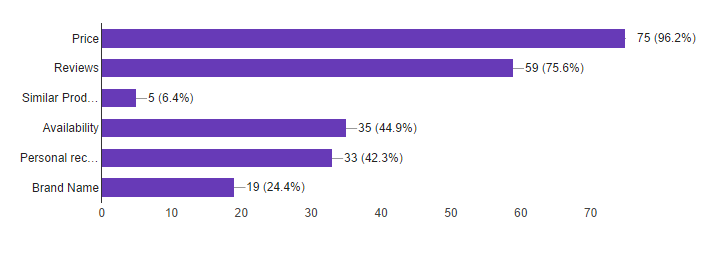
\includegraphics[width=0.9\columnwidth]{figures/ShoppingFactors}
	\caption{Most important factors in making shopping decisions}
	\label{figures:ShoppingFactors}
\end{figure}

 \subsection{Methodology}
We distributed a preliminary survey over social media to identify important aspects of customers' in-store and online shopping experiences and received responses from 78 participants. We asked participants to identify the three most important pieces of information involved their shopping decisions, what they did and did not like about existing in-store and online shopping experiences, and ways they currently use technology in shopping. \todo{does this feel like a reasonable synopsis?}  \todo{JRB: Yes, except I would like to know if these were open-ended questions or not.}
We used the responses from our online survey to
%isolate -- JRB: WC?
identify 
factors of in-store and online shopping that were most important to our participants.  Relevant to the current paper, we asked participants if they use a mobile device while in-store to make purchasing decisions, and to select important factors from a list we provided. Figure \ref{figures:ShoppingFactors} details participants' responses when prompted for their three most important factors in making shopping decisions. Using open-ended questions, we asked participants what they liked the most and least about shopping online and in store. We clustered responses based on similarity, resulting in the findings below.

%% JRB -- Removed, not needed: \subsection{Findings}
Participants appreciate the immediacy and physical interaction with products in a store, but cited drawbacks included the inability to comparison shop, to get the lowest price and/or feeling that they are paying too much, and store staff trying to influence purchase decisions.  Participants appreciate the freedom from store location and hours, \todo{I'm not sure what "freedom from store location and hours" means - EH} \todo{JRB: Ditto.} and time-to-completion of online shopping, \todo{I'm confused as to whether you're talking about things participants appreciate about in-store shopping or about online shopping} but said they dislike the shipping charges and wait times associate with online shopping. We also found that users are willing to spend more time researching more expensive products. These findings provided a foundation from which we engage in our design work in phases 2 and 3.


\section{Phase 2: Low Fidelity Prototype}
\subsection{Methodology}
We used the results from our preliminary survey to design two sketch-based low fidelity prototypes of an AR system containing aspects of in-store and online shopping experiences that participants identified as important.  We can bring critical factors of online experiences, such as access to reviews and ease of comparison, into the store environment while preserving aspects of in-store decision making, such as being ``hands-on with the product'' and leaving the store with the product. We hypothesized that an augmented reality application that supplemented a traditional in-store experience with immediate access to core aspects of online shopping would improve consumer's confidence in their purchasing decisions. \todo{replace the last bit of this sentence with what was actually tested}

\todo[inline]{JRB: The paragraph below talks about one prototype. I think you should say that you had two. One prototype for interaction concept.}
We tested our hypothesis in a think-aloud study using our sketch-based prototypes as a design prompt. \todo{JRB: Formative design work and evaluation do not have to be hypothesis driven, and often aren't. Instead they are exploratory. If you are feeling encumbered by the "hypothesis" language, we can reword. Just let me know.} The prototypes consisted of online content drawn as AR menus on transparency sheets and overlaid onto an image of an electronics store. Participants interacted with each of the two prototypes, in a random order, and were allowed to navigate through a electronics retail experience. We used to two prototypes to make a comparison between a menu-based, hierarchically structured user experience, and a context-aware virtual overlays of product information. \todo{what specific AR components were tested here (e.g., reviews, product comparisons, specs, etc.)? What were your measures here (e.g., confidence in the decision, time to decision, etc.)} \todo{JRB: How did you analyze the data from this phase?}
\todo[inline]{figure of paper prototype}

\subsection{Findings}
We recruited three participants from campus for this study. Generally, participants were more receptive to quick and less information than to a fuller, menu-based approach. Participants stated that the ability to see specifications of two different laptops in the same view is valuable in decision-making. Participants also expressed a desire to toggle display of content. One participant identified demos as a useful application of augmented reality in retail.

\section{Phase 3: High Fidelity Prototype}

\subsection{Methodology}
We used the responses from the low fidelity prototype study to design a fully immersive StoAR prototype for use in head-mounted displays. Because we did not have access to a retail testing environment, we simulated a retail display in virtual reality based on configurations found in a local retail outlet. We then added an augmented reality interface to the simulation to provide review and price information, depicted in Figure 2.\todo{briefly describe the important pieces informed by the low-fi study} \todo{Add figure according to CHI LBW format} While our use of a VR store simulation removes immediate access to real life product found in a real world store, the fully immersive environment allowed us to closely control the relationship between the prototype AR interfaces and simulated products. %and reduced the environmental complexity to allow participants to focus solely on the prototype implementation. 

We used a post-hoc survey to measure people's responses to the immersive prototype. Participants first freely navigated the virtual representation of a store augmented with static content containing information about each device. 
%Given space constraints, the track pad on one of the Vive's controllers was employed for users to navigate within the scene.
After navigating the scene, participants reported their perceptions of the prototype's usability, potential impact on decision-making, utility of individual design components, perceived trade-offs compared to existing technologies and potential limitations of the approach. They also provided feedback on additional applications where they envisioned using mixed reality experiences for decision making. As with the initial online survey, we aggregated the qualitative feedback provided by users.
%The survey asked for specific product-domains to which our system could be applied (i.e. electronics, furniture, books).  


\subsection{Findings}
We recruited 20 participants from a local research expo to complete this study. Participants said they envision using this platform for comparison shopping, quickly seeing reviews, prices, and product specifications, and visual demonstrations of product use. Lower depth of product information was provided as a tradeoff of the system. Participants expressed concern about digital content distracting them from the physical environment. Having presented them with laptops, we asked participants for what other products they think augmented reality could aid them in decision-making, with the results shown in Figure 3. \todo{MW: Games, toys, furniture, and clothing.  Honestly, this finding doesn't really line up with anything else, unless we start drawing conclusions about "They said furniture because of potential for visualizations" or something like that. We have a figure if we want to keep this point.}

We prompted participants for additional features of a retail augmented reality system such as this one. Participants detailed several expected interactions with the static content provided. Aligning with feedback from the low-fidelity prototypes, participants wanted to keep information within a single view such that they could comparison shop. With the way content was provided in the high-fidelity prototype, users would need to turn around or walk toward another laptop to view its associated information. Participants expressed that they want to compare prices of the same product against other stores' prices. If presented with the option, participants said they would consider purchasing from another source.

\section{Discussion}

\subsection{Merging Physical \& Virtual Experiences}
We found preliminary evidence that AR can merge online and in-store experiences to benefit the consumer by preserving aspects of in-store shopping that people enjoy while adding preferred aspects of online experiences.  In the initial survey, participants cited the ability to find the best price and access reviews as the most important reasons to use technology in shopping. However, the participants who interacted with the StoAR prototypes indicated that it would allow them to better analyze product specs \emph{in situ}, compare reviews and ratings against their own experiences, and mediate their interactions with physical products through virtual demos.

These findings align well with prior studies in e-commerce, which demonstrate the utility of price and product comparison in online shopping. Our design-based approach confirmed important aspects of online shopping shared by participants in the initial survey. We also found that people's perceptions of how AR might benefit their decision making evolved as the prototypes grew more sophisticated. These shifting perceptions suggest that using prototypes as design prompts is beneficial for helping people envision how AR experiences might differ from conventional methods. 

\subsection{New Opportunities for Blended Experiences}
We also found evidence that AR might enable unique kinds of decision support that neither physical nor virtual experiences alone can provide. For example, our high fidelity prototype provided static summaries of the product data identified as critical in the low fidelity study. However, in the high fidelity prototype, participants expressed an additional desire to interact with the system, such as the ability to virtually ``pin'' relevant information for easy access as they navigated the store or access to specific details on demand. Participants also reported a desire to use AR to simulate their own at-home context or use case for a particular product, particularly room design and game previews. 
%MW: Removed for space
%They felt such features would allow them to ``look at products without being at a brick and mortar store,'' prioritizing the convenience of online shopping. 
The ability to explore these simulations to virtually unbox a product would provide additional information inaccessible in traditional experiences.

These findings collectively suggest that designing mixed reality applications is not as simple as blending the best aspects of both the virtual and physical experiences. AR technologies allow new methods for supporting decision making not afforded by purely physical or virtual methods. Instead, designers must critically reflect on how AR may effectively mediate novel kinds of interactions to transcend traditional approaches and provide consumers with new forms of decision support. 
%MW: Removed for space
%Future work can explore how the capabilities of these technologies and properties of the target domain and task might inform novel AR experiences.
%Not as simple as drag and drop: need for understanding at a glance communication to provide effective delivery.  

\subsection{Designing for Effective Communication}
Participants in the study frequently commented on the need to carefully limit the amount of information provided by the interface. Participants want to be empowered with pertinent information, but it must be easily digestible to avoid interfering with the immediacy of the in-store experience. They expressed some concern about trying to process too much information and about the display being too distracting, inhibiting their ability to navigate the physical store. Instead, participants preferred sparsely presented information in-context, allowing them to access relevant review and product information at a glance. 

%MW: 5:58 Submission--this is commented out. Would like to put back in.
%Future systems will benefit from a better understanding of the balance between information presented and visual space consumed. Our findings identify a need to understand how AR systems might balance communicative power with interaction to deliver necessary information. A lack of consensus amongst participants as to what information is ``necessary'' suggests opportunities for designing intelligent interfaces and customized experiences not available in real world environments to support individual decision making. 
%modes for interaction, interface design, customization? Also, balance needs of the consumer and producer: how can we empower users while working within the constraints of the available params

\subsection{Limitations \& Future Work}
Our high fidelity prototype used a simulated store display rather than a real world environment.  While this approach allowed us to conduct a preliminary evaluation of the prototype without the added complexity of instrumentation or physical obstacles, it also limits our ability to fully characterize the affordances of our prototype in practice. Previous work such as et al. \cite{macintyre2004dart} deals with effectively prototyping augmented reality experiences. Prototyping in the intended medium yields a more rapid prototyping process than a separate device or framework.
%MW: Removed...you know why
%While we believe that the design guidance provided by our work can inform effective blended experiences, we also realize that further refining and implementing StoAR in full AR is a critical next step. 
%MW: Definitely won't include this text.  But it's good content to hang onto just in case.
%Even if not a misconception, this finding points toward use of the intended hardware in prototyping for augmented reality.  If we used an augmented reality head-mounted display, we could test for safety in addition to usability.
%This prototype represents a physical store with augmented reality content.  Several users provided feedback indicating that they did not understand the concept of prototyping augmented reality in virtual reality.  In some cases, users gave feedback perceiving the system as a virtual store to virtually navigate.  
%More effective means of prototyping augmented reality, ideally using the system's intended hardware, would eliminate some of these misconceptions. \todo{frame this in terms of trade-offs: vr gives nearly full control, but removes many of the complexities of experiencing these systems in practice. Here, it allows us to gain a sense of how people would respond to the system alone, but future work is needed to understand how these responses generalize to the noisy contexts of stores}  In some cases, these concerns may have stemmed from a lack of understanding, as users may have thought their entire view of their surroundings would be blocked by a virtual reality head-mounted display.  

In our first survey, many participants reported that they use a mobile device while in a physical store. This approach allows for people to retrieve in-depth information \emph{in situ}, but it also requires significant effort to locate and compare relevant information on the fly. Participants reported that they ``like the idea of hands-free/ambient information'' offered by HMDs over mobile devices, but were concerned about the legibility of the information presented in AR. Our future work will directly compare traditional mobile devices to the StoAR approach to better understand the trade-offs of blended and parallel methods for decision making. 

\section{Conclusion}
% First, revisit the rq and findings
We explored how understanding the trade-offs of parallel physical and virtual experiences could inform mixed reality applications in the context of retail shopping. Our findings suggest that participants appreciated the ability of mixed reality experiences to offer more rapid access to information about products while preserving the physical interactions offered by in-store experiences. Using a design-based methodology allowed potential users to envision ways that AR technologies might enable new experiences beyond those offered by physical or virtual methods alone, such as mediating evaluative interactions with products like guided demos or simulated placement.  
% Then, introduce the synthesis
Our findings, gathered throughout the design process, highlight the potential for AR in retail environments and open new avenues for understanding how we might effectively derive new AR experiences from existing processes.

\balance{} 

% \bibliographystyle{ACM-Reference-Format-Journals}
\bibliographystyle{SIGCHI-Reference-Format}
% \bibliographystyle{acm}
\bibliography{sample}


\end{document}

%%% Local Variables:
%%% mode: latex
%%% TeX-master: t
%%% End:
